\chapter{Propuesta de Proyecto}
\label{sec:propuesta}

Para el éxito de todo proyecto, es necesario desarrollar un estudio de factibilidad, que evalúe la viabilidad técnica, económica y operativa de la iniciativa propuesta.  Este análisis exhaustivo proporciona una base sólida para la toma de decisiones informadas y la asignación adecuada de recursos, minimizando los riesgos y maximizando las oportunidades de éxito.

\begin{comment}
En esta sección se describe la propuesta del perfil de tesis/proyecto de grado. Dicha propuesta debe estar basada en el marco teórico, a fin de facilitar la comprensión del lector acerca de la innovación tecnológica que el candidato pretende llevar a cabo durante el desarrollo de su tesis/proyecto de grado.
La propuesta de tesis/proyecto de grado debe hacer uso de diversos recursos, tales como: ecuaciones, diseños CAD, circuitos de diferente índole, tablas, figuras, entre otras que permitan describir con efectividad los objetivos que desea alcanzar en caso de ser aprobado su perfil.
Este apartado o sección, por tanto, es de gran importancia y debe ser detallado con la objetividad y el profesionalismo que se espera de un candidato al grado de ingeniero.
\end{comment}

%---------------------------------------------------------------------------------------------
%---------------------------------------------------------------------------------------------
\section{Análisis de Costos}

El análisis del proyecto se ha llevado a cabo desde dos perspectivas fundamentales: el costo de desarrollo del proyecto de grado y la proyección de los ingresos y beneficios esperados mediante la implementación del modelo de Software como Servicio (SaaS por sus siglas en inglés) en una estructura empresarial completamente virtual, donde cada programador involucrado utiliza su equipo personal para el desarrollo.

%---------------------------------------------------------------------------------------------
\subsection{Costos de Desarrollo}
La estimación del costo de desarrollo para el proyecto se basó en el modelo COCOMO intermedio (\cite{basavaraj2008empirical}). Este modelo calcula el esfuerzo necesario para desarrollar software considerando el tamaño del programa y varios factores que influyen en los costos, como atributos del producto, hardware y personal. Para una evaluación más detallada de estos factores, se puede consultar la tabla de ponderación de impulsores en el anexo \ref{sec:cocomo}. \\
Para la estimación del numero de lineas de código se utilizó el prototipo de uno de los módulos del programa. El prototipo consta de aproximadamente 600  efectivas de código. Asumiendo que el desarrollo es orgánico y que todos los módulos tendrán una longitud similar y el alcance del proyecto de grado se limita a por lo menos tres módulos: Se espera con 1800 lineas de código. Por otro lado, de acuerdo a \textcite{glassdoor2024} el salario promedio de desarrolladores junior en Bolivia es de Bs. 6000.\\ \indent
El modelo aplicado al proyecto estima inicialmente un esfuerzo de $5.93$ persona-mes, que representa el trabajo requerido sin ajustar los factores específicos del proyecto. Tras aplicar estos factores de ajuste, el esfuerzo aumenta a $8.76$ persona-mes, reflejando un incremento significativo debido a las particularidades del proyecto. El tiempo total estimado para el desarrollo es de $5.70$ meses, sugiriendo que el proyecto se completará en menos de medio año. Para cumplir con este plazo, se necesita un equipo promedio de aproximadamente $1.54$ personas. \\
\begin{equation}\label{eq:costo_desarrollo}
    Costo\ Desarrollo\ MVP = Esfuerzo(Persona-Mes) \times Salario(Bs/Persona-Mes)
\end{equation}

\begin{equation*}
    Costo\ Desarrollo\ MVP = 8.76 \times Bs.6000 = Bs.52,560.00
\end{equation*}
Finalmente, con la ecuación \ref{eq:costo_desarrollo} se calcula el costo de desarrollo como el producto del esfuerzo en persona-mes, el salario mensual y el numero de desarrolladores idealmente requeridos. Resultando en un costo estimado de desarrollo de Bs.$52,560.00$. Adicionalmente, caso se evalué el proyecto completo automatizando las siete actividades de la Tabla \ref{tab:tabla_requisitos_nts_009}, por medio de la misma metodología se concluye que el proyecto completo tendría un costo de Bs.$245,069.81$.

%---------------------------------------------------------------------------------------------
\subsection{Costos de Infraestructura}

En el contexto del modelo SaaS, es crucial evaluar y seleccionar adecuadamente la infraestructura tecnológica sobre la cual se desplegará el software. Este modelo requiere una plataforma robusta y escalable que permita no solo un buen desempeño sino también una gestión eficiente de los costos a lo largo del tiempo. Para seleccionar la plataforma más adecuada para el proyecto se considerando diversos criterios técnicos y financieros. La Tabla \ref{tab:sel_servicios} presenta una matriz de evaluación que compara los tres principales proveedores de servicios en la nube: Amazon Web Services (AWS), Google Cloud y Microsoft Azure. En función de varios criterios ponderados. Asumiendo AWS como servicio a utilizar y se proyectan los costos de este servicio al cambio de Bs.6.96 por dolar.

\begin{table}[htb]
    \caption{Matriz de Selección de Servicios de Computación en la Nube}
    \label{tab:sel_servicios}
    \centering
    \small
    \begin{tabularx}{\textwidth}{|l|X|X|X|X|X|}
    \hline
    \textbf{Criterios} & \textbf{Peso} & \textbf{AWS} & \textbf{Google Cloud} & \textbf{Microsoft Azure} \\
    \hline
    \textbf{Rendimiento} & 15\% &
    \begin{tabular}{@{}p{0.9cm}|p{2.4cm}@{}}
    5 & 0.75 \\
    \end{tabular}
    &
    \begin{tabular}{@{}p{0.9cm}|p{2.4cm}@{}}
    4 & 0.60 \\
    \end{tabular}
    &
    \begin{tabular}{@{}p{0.9cm}|p{2.4cm}@{}}
    4 & 0.60 \\
    \end{tabular}
    \\
    \hline
    \textbf{Confiabilidad} & 15\% &
    \begin{tabular}{@{}p{0.9cm}|p{2.4cm}@{}}
    5 & 0.75 \\
    \end{tabular}
    &
    \begin{tabular}{@{}p{0.9cm}|p{2.4cm}@{}}
    5 & 0.75 \\
    \end{tabular}
    &
    \begin{tabular}{@{}p{0.9cm}|p{2.4cm}@{}}
    5 & 0.75 \\
    \end{tabular}
    \\
    \hline
    \textbf{Escalabilidad} & 15\% &
    \begin{tabular}{@{}p{0.9cm}|p{2.4cm}@{}}
    5 & 0.75 \\
    \end{tabular}
    &
    \begin{tabular}{@{}p{0.9cm}|p{2.4cm}@{}}
    5 & 0.75 \\
    \end{tabular}
    &
    \begin{tabular}{@{}p{0.9cm}|p{2.4cm}@{}}
    5 & 0.75 \\
    \end{tabular}
    \\
    \hline
    \textbf{Seguridad} & 15\% &
    \begin{tabular}{@{}p{0.9cm}|p{2.4cm}@{}}
    5 & 0.75 \\
    \end{tabular}
    &
    \begin{tabular}{@{}p{0.9cm}|p{2.4cm}@{}}
    5 & 0.75 \\
    \end{tabular}
    &
    \begin{tabular}{@{}p{0.9cm}|p{2.4cm}@{}}
    5 & 0.75 \\
    \end{tabular}
    \\
    \hline
    \textbf{Costo} & 20\% &
    \begin{tabular}{@{}p{0.9cm}|p{2.4cm}@{}}
    3 & 0.60 \\
    \end{tabular}
    &
    \begin{tabular}{@{}p{0.9cm}|p{2.4cm}@{}}
    4 & 0.80 \\
    \end{tabular}
    &
    \begin{tabular}{@{}p{0.9cm}|p{2.4cm}@{}}
    3 & 0.60 \\
    \end{tabular}
    \\
    \hline
    \textbf{Soporte} & 10\% &
    \begin{tabular}{@{}p{0.9cm}|p{2.4cm}@{}}
    5 & 0.50 \\
    \end{tabular}
    &
    \begin{tabular}{@{}p{0.9cm}|p{2.4cm}@{}}
    4 & 0.40 \\
    \end{tabular}
    &
    \begin{tabular}{@{}p{0.9cm}|p{2.4cm}@{}}
    5 & 0.50 \\
    \end{tabular}
    \\
    \hline
    \textbf{Facilidad de uso} & 10\% &
    \begin{tabular}{@{}p{0.9cm}|p{2.4cm}@{}}
    4 & 0.40 \\
    \end{tabular}
    &
    \begin{tabular}{@{}p{0.9cm}|p{2.4cm}@{}}
    4 & 0.40 \\
    \end{tabular}
    &
    \begin{tabular}{@{}p{0.9cm}|p{2.4cm}@{}}
    3 & 0.30 \\
    \end{tabular}
    \\
    \hline
    \textbf{Total} & & 4.50 & 4.45 & 4.25 \\
    \hline
    \end{tabularx}
    \end{table}
    

\subsubsection{Servidores y Almacenamiento}\hfill\\ 
\indent
Los costos de servidores y almacenamiento en AWS pueden variar significativamente según las necesidades específicas del proyecto. Para este análisis, se asume un uso moderado de los servicios, considerando un entorno de desarrollo, pruebas y producción. 

\begin{itemize}[noitemsep,topsep=0pt,parsep=0pt,partopsep=0pt]
    \item Elastic Compute Cloud (EC2): Utilizado para alojar los servidores de aplicaciones. Se estima que se utilizarán instancias t2.medium para el entorno de desarrollo y pruebas, y instancias m5.large para el entorno de producción. Asumiendo un uso continuo, los costos estimados son:
    \begin{itemize}[noitemsep,topsep=0pt,parsep=0pt,partopsep=0pt]
    \item Desarrollo y Pruebas: 2 instancias t2.medium a $0.0464$ por hora cada una.
    \item Producción: 1 instancia m5.large a $0.096$ por hora.
    \end{itemize}
    \begin{equation*}\label{eq_costo_ec2}
    Costo\ EC2\ mensual = (720) ( 2 \times \$0.0464 + \$0.096) = \$135.94 = Bs.946.14
    \end{equation*}
    \item Simple Storage Service (S3): Utilizado para almacenamiento de objetos, como archivos estáticos y backups. Se estima un uso de 500 GB por mes a \$0.023 por GB.
    \begin{equation*}\label{eq_costo_s3}
    Costo\ S3\ mensual = 500 \times \$0.023 = \$11.50 = Bs.80.04
    \end{equation*}
    \item Relational Database Service (RDS): Utilizado para la base de datos relacional. Se asume el uso de una instancia db.t3.medium para el entorno de producción a \$0.0416\$ por hora.
    \begin{equation*}\label{eq_costo_rds}
    Costo\ RDS\ mensual = 0.0416 \times 720 = \$29.95 = Bs.208.45
    \end{equation*}
\end{itemize}

\subsubsection{Red y Seguridad}\hfill\\ 
\indent
Además de los costos de servidores y almacenamiento, es importante considerar los costos asociados a la red y la seguridad.

\begin{itemize}[noitemsep,topsep=0pt,parsep=0pt,partopsep=0pt]
\item Transferencia de Datos: Se estima un tráfico mensual de 1 TB (entrada y salida), con un costo de \$0.09 por GB para los primeros 10 TB.
\begin{equation*}\label{eq_transf_datos}
Costo\ transferencia\ de\ datos\ mensual = 1024 \times 0.09 = \$92.16 = Bs.641.43
\end{equation*}
\item Servicios de Seguridad: Incluye AWS WAF (\textit{Web Application Firewall}) y Amazon GuardDuty. Se estima un costo mensual combinado de aproximadamente \$50 (Bs. 348).
\end{itemize}

\subsubsection{Costos Totales de Infraestructura}\hfill\\ 
\indent
Se concluye este análisis tras haber estimado los costos totales para la infraestructura propuesta. Estos costos incluyen los gastos mensuales asociados con los servidores, la red y la seguridad, esenciales para mantener las operaciones en la nube a través de AWS. A continuación, se detalla el cálculo de estos costos:

\begin{table}[ht]
    \caption{Detalle de Costos Mensuales de Infraestructura.}
    \label{tab:costos_infraestructura}
    \centering
    \begin{tabularx}{\textwidth}{|X|r|} 
        \hline
        \textbf{Concepto} & \textbf{Monto (Bs)} \\ \hline
        Servidores (EC2) & 946.14 \\ 
        Almacenamiento (S3) & 80.04 \\ 
        Base de Datos (RDS) & 208.45 \\ 
        Transferencia de datos & 641.43 \\ 
        Servicios de Seguridad & 348.00 \\ \hline
        \textbf{Total Costo de Infraestructura} & \textbf{2,224.06} \\ \hline
    \end{tabularx}
\end{table}

Así, el costo mensual de la infraestructura mediante AWS se calcula en $Bs.2,224.06$. Es decir, el costo anual estimado de infraestructura en AWS es de $Bs.26,668.72$. Es importante destacar que estos costos pueden variar según el uso real y la optimización de recursos a lo largo del tiempo.

%---------------------------------------------------------------------------------------------
\subsection{Gastos Legales}

La creación de una sociedad implica una serie de gastos legales necesarios para cumplir con las normativas vigentes y asegurar su correcta constitución. Estos gastos incluyen tarifas administrativas, honorarios profesionales y otros costos relacionados.En la Tabla \ref{tab:costos_legales} se detallan los costos legales asociados a la creación de la sociedad.

\begin{table}[ht]
    \centering
    \caption{Gastos legales de creación de la sociedad.}
    \label{tab:costos_legales}
    \begin{tabularx}{\textwidth}{|X|r|} 
        \hline
        \textbf{Descripción} & \textbf{Costo (Bs)} \\ \hline
        Arancel de Seprec & 455 \\ 
        Publicación Gaceta & 192 \\ 
        Balance de apertura del contador & 200 \\ 
        Gobierno autónomo municipal Santa Cruz & 150 \\ 
        Honorarios notario & 500 \\ 
        Honorarios abogado & 3500 \\ \hline
        \textbf{TOTAL} & \textbf{4997} \\ \hline
    \end{tabularx}
\end{table}

%---------------------------------------------------------------------------------------------
\subsection{Inversión Total Inicial}

En la Tabla \ref{tab:inversion_total}, se presenta la inversión total inicial necesaria para el proyecto. Según los cálculos, la inversión total inicial estimada para iniciar el proyecto asciende a $Bs.59,781.06$. Este monto abarca todos los aspectos indispensables para el desarrollo, implementación y operación inicial del software bajo el modelo SaaS.

\begin{table}[ht]
    \centering
    \caption{Inversión Total Inicial}
    \label{tab:inversion_total}
    \begin{tabularx}{\textwidth}{|X|r|}
        \hline
        \textbf{Concepto} & \textbf{Costo (Bs)} \\
        \hline
        Costo de Desarrollo & 52,560.00 \\
        Costos de Infraestructura & 2,224.06 \\
        Gastos Legales & 4,997.00 \\
        \hline
        \textbf{Total} & \textbf{59,781.06} \\
        \hline
    \end{tabularx}
\end{table}

%---------------------------------------------------------------------------------------------
%---------------------------------------------------------------------------------------------
\section{Evaluación de Proyecto de Inversión}
La evaluación de un proyecto de inversión es fundamental para determinar su viabilidad y potencial de rentabilidad. En esta sección, se abordan tres elementos clave: la comparación costo-beneficio, el Valor Actual Neto (VAN) y la Tasa Interna de Retorno (TIR). Estos indicadores financieros proporcionan una comprensión profunda de los ingresos proyectados frente a los costos, la rentabilidad esperada descontada a valor presente y la eficiencia general del proyecto. Este análisis integral permite tomar decisiones informadas y estratégicas sobre la inversión.

%---------------------------------------------------------------------------------------------
\subsection{Comparación Costo Beneficio}

El análisis financiero del proyecto asumiendo el modelo de negocio SaaS con la proyección del proyecto completo. Se calculó la relación entre los ingresos y costos anuales asumiendo un programador junior contratado para realizar el desarrollo y mantenimiento continuo del sistema; Ademas que inicialmente que se capta al 10\% del mercado potencial como usuario mismos que incrementan según la tasa de incremento de profesionales SySO anual del $58.8\%$ visible en la Figura \ref{fig:profesionales_syso_registrados}. Los resultados de la proyección se presentan en la Tabla \ref{tab:proyeccion_financiera} en la que se utilizó un un costo por membresía de Bs.70. La relación costo-beneficio mejora significativamente a lo largo de los años, comenzando en 1.00 en el primer año y alcanzando 18 en el quinto año. Esto indica que, para el quinto año, por cada boliviano invertida, se generan alrededor de 18 bolivianos en ingresos.

\begin{table}[htb]
    \caption{Proyección financiera del proyecto bajo el modelo SaaS.}
    \label{tab:proyeccion_financiera}
    \centering
    \begin{tabularx}{\textwidth}{|l|r|>{\raggedleft\arraybackslash}X|>{\raggedleft\arraybackslash}X|>{\raggedleft\arraybackslash}X|r|}
        \hline
        \thead{Año} & \thead{Usuarios\\Mensuales} & \thead{Gastos\\Anuales (Bs)}  & \thead{Ingresos\\Anuales (Bs)}  & \thead{Balance\\Anual (Bs)} & \thead{C/B} \\ \hline
        0 & 0 & 276,755.53 & 00.00 & -276,755.53 & 0.00 \\ \hline
        1 & 330 & 98,688.72 & 277,200.00 & 178,511.28 & 2.81 \\ \hline
        2 & 525 & 98,688.72 & 441,000.00 & 342,311.28 & 4.47 \\ \hline
        3 & 834 & 98,688.72 & 700,560.00 & 601,871.28 & 7.10 \\ \hline
        4 & 1325 & 98,688.72 & 1,113,000.00 & 1,014,311.28 & 11.28 \\ \hline
        5 & 2104 & 98,688.72 & 1,767,360.00 & 1,668,671.28 & 17.91 \\ \hline
    \end{tabularx}
\end{table} 

%---------------------------------------------------------------------------------------------
\subsection{Valor Actual Neto}
El Valor Actual Neto (VAN) es una medida financiera que calcula la diferencia entre el valor presente de los flujos de efectivo entrantes y salientes de un proyecto. Se calcula descontando los flujos de caja futuros a una tasa de descuento y restando la inversión inicial. Para este proyecto, se utiliza una tasa de descuento del 10\%. 

\begin{equation}
    \label{eq:VAN}
    VAN = \sum \frac{ganancias}{(1+K)^{n}} - \sum \frac{costos}{(1+K)^{n}}
\end{equation}

\begin{equation*}
    VAN =  2,135,932.70
\end{equation*}

El VAN se calcula restando los flujos de efectivo descontados de los costos descontados, lo que da como resultado un VAN de 2,464,402.58. Esto indica que, después de descontar los flujos de efectivo futuros y la inversión inicial, el proyecto en cuestión generaría un valor adicional de 2,464,402.58 en términos de valor presente neto. Este resultado sugiere que el proyecto tiene un potencial de rentabilidad positivo y podría ser una inversión atractiva.

%---------------------------------------------------------------------------------------------
\subsection{Tasa Interna de Retorno}
La Tasa Interna de Retorno (TIR) es un indicador financiero utilizado para evaluar la rentabilidad de una inversión. Representa la tasa de descuento que iguala el VAN de una serie de flujos de caja a cero. En otras palabras, la TIR es la tasa de interés que hace que el valor presente de los ingresos futuros de una inversión sea igual al costo inicial de la misma.
\begin{equation}
    \label{eq:TIR}
    VAN = \sum_{t=1}^{n} \frac{F_t}{(1+TIR)^{t-1}} - I = 0
\end{equation}
\indent
En la ecuación \ref{eq:TIR}, $F_t$ son los flujos de caja en el periodo $t$, $n$ es el número total de periodos, e $I$ es la inversión inicial. La misma se resuelve iterativamente, ya que no tiene una solución algebraica directa, especialmente cuando los flujos de caja no son constantes. El valor de la TIR es útil porque permite comparar la rentabilidad de diferentes proyectos de inversión. En general, un proyecto se considera aceptable si su TIR es mayor que la tasa mínima de rendimiento requerida o el costo de oportunidad del capital. En el contexto del proyecto evaluado, se ha determinado que la TIR es del 112\%. Este valor indica una alta rentabilidad del proyecto, ya que la tasa de retorno esperada es significativamente superior al costo de capital típico en muchos sectores.

%---------------------------------------------------------------------------------------------
\subsection{Conclusión}
La evaluación del proyecto de inversión mediante la comparación costo-beneficio, el VAN y el TIR revela una perspectiva prometedora. La proyección financiera muestra una mejora constante en la relación costo-beneficio, culminando en una relación de 18:1 para el quinto año. El VAN positivo de 2,135,932.70 sugiere que el proyecto no solo recuperará la inversión inicial sino que también generará un valor neto significativo. La TIR del 112\% indica una alta rentabilidad, superando ampliamente las tasas de retorno estándar en la industria. Estos resultados combinados apoyan la viabilidad y rentabilidad del proyecto, recomendando su implementación como una inversión estratégica y beneficiosa.

%---------------------------------------------------------------------------------------------
%---------------------------------------------------------------------------------------------
\section{Análisis de Competidores}

Se realizó un análisis de competidores para identificar oportunidades y amenazas en el mercado, así como para comprender la posición relativa del producto propuesto frente a sus rivales, lo cual permite formular estrategias efectivas y diferenciarse en el mercado del software de gestión de salud y seguridad. 

A nivel mundial, el mercado del software de salud y seguridad ocupacional se compone de dos tipos predominantes: soluciones basadas en la nube y soluciones basadas en la web. El software basado en la nube se refiere a un sistema al que se accede a través de internet, donde los datos se almacenan y procesan en servidores remotos. Ofrece mayor flexibilidad, escalabilidad y accesibilidad. Por otro lado, el software basado en la web funciona a través de un navegador web, requiriendo conectividad a internet. Proporciona comodidad y facilidad de uso, ya que los usuarios pueden acceder al software desde cualquier dispositivo con un navegador. Subdividiéndose por aplicación en: `Grandes empresas' y `Pequeñas y Medianas Empresas' (PyME). Las grandes empresas necesitan software que gestione eficazmente la salud y seguridad ocupacional en diversos departamentos y ubicaciones, debido a su estructura compleja y mayor cantidad de empleados. Las PyMEs, en cambio, requieren soluciones rentables que cubran sus necesidades de gestión de salud y seguridad. Por lo tanto, el mercado ofrece aplicaciones de software adaptadas a ambos segmentos para cumplir con sus requisitos específicos y asegurar la conformidad con las normativas de salud y seguridad (\cite{KingpinMarketResearch}).

Rápidamente la Figura~\ref{fig:visitas_por_dominio} permite observar que las tres compañías con mayor ocupación del mercado en lo que a tráfico de red se refiere son \textit{sitedocs}, \textit{donesafe} y \textit{everbridge}. Estas tres empresas juntas representan más del 50\% del tráfico total, destacando su fuerte presencia y dominio en el mercado (\cite{SEMrushMarketExplorer}).

\begin{figure}[htb]
    \centering
    \fbox{
        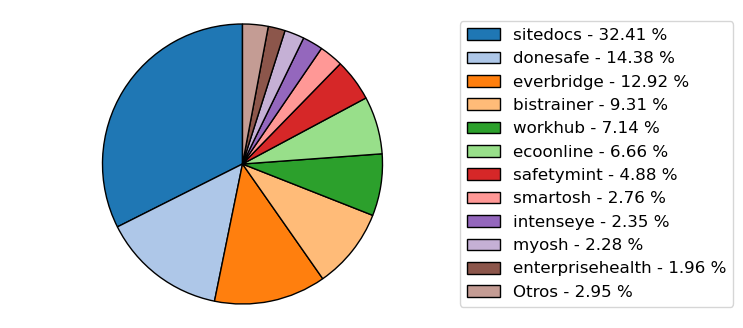
\includegraphics[width=0.95\linewidth]
        {images/marcopractico/planificacion/visitas_por_dominio.png}
    }
    \caption{Participación de Mercado de los Principales Competidores}
    \vspace{-0.2cm}
    \footnotesize{{Elaboración propia a partir de datos obtenidos por medio de ``\textit{\citefield{SEMrushMarketExplorer}{title}}'' (\citeyear{SEMrushMarketExplorer}).}}
    \label{fig:visitas_por_dominio}
\end{figure}

A su vez, la matriz ilustrada en la Figura~\ref{fig:MatrizCompetidores}, divide los dominios en cuatro categorías: Jugadores de nicho, agentes de cambio, líderes y jugadores establecidos. El eje X representa el volumen total de tráfico que reciben los dominios, mientras que el eje Y muestra el porcentaje de crecimiento del tráfico total. Cada punto en el gráfico representa un dominio y su trayectoria de crecimiento durante el período seleccionado. Las líneas que conectan los puntos iniciales y finales muestran el cambio en el tráfico y la tasa de crecimiento a lo largo del tiempo.

\begin{figure}[htb]
    \centering
    \fbox{
        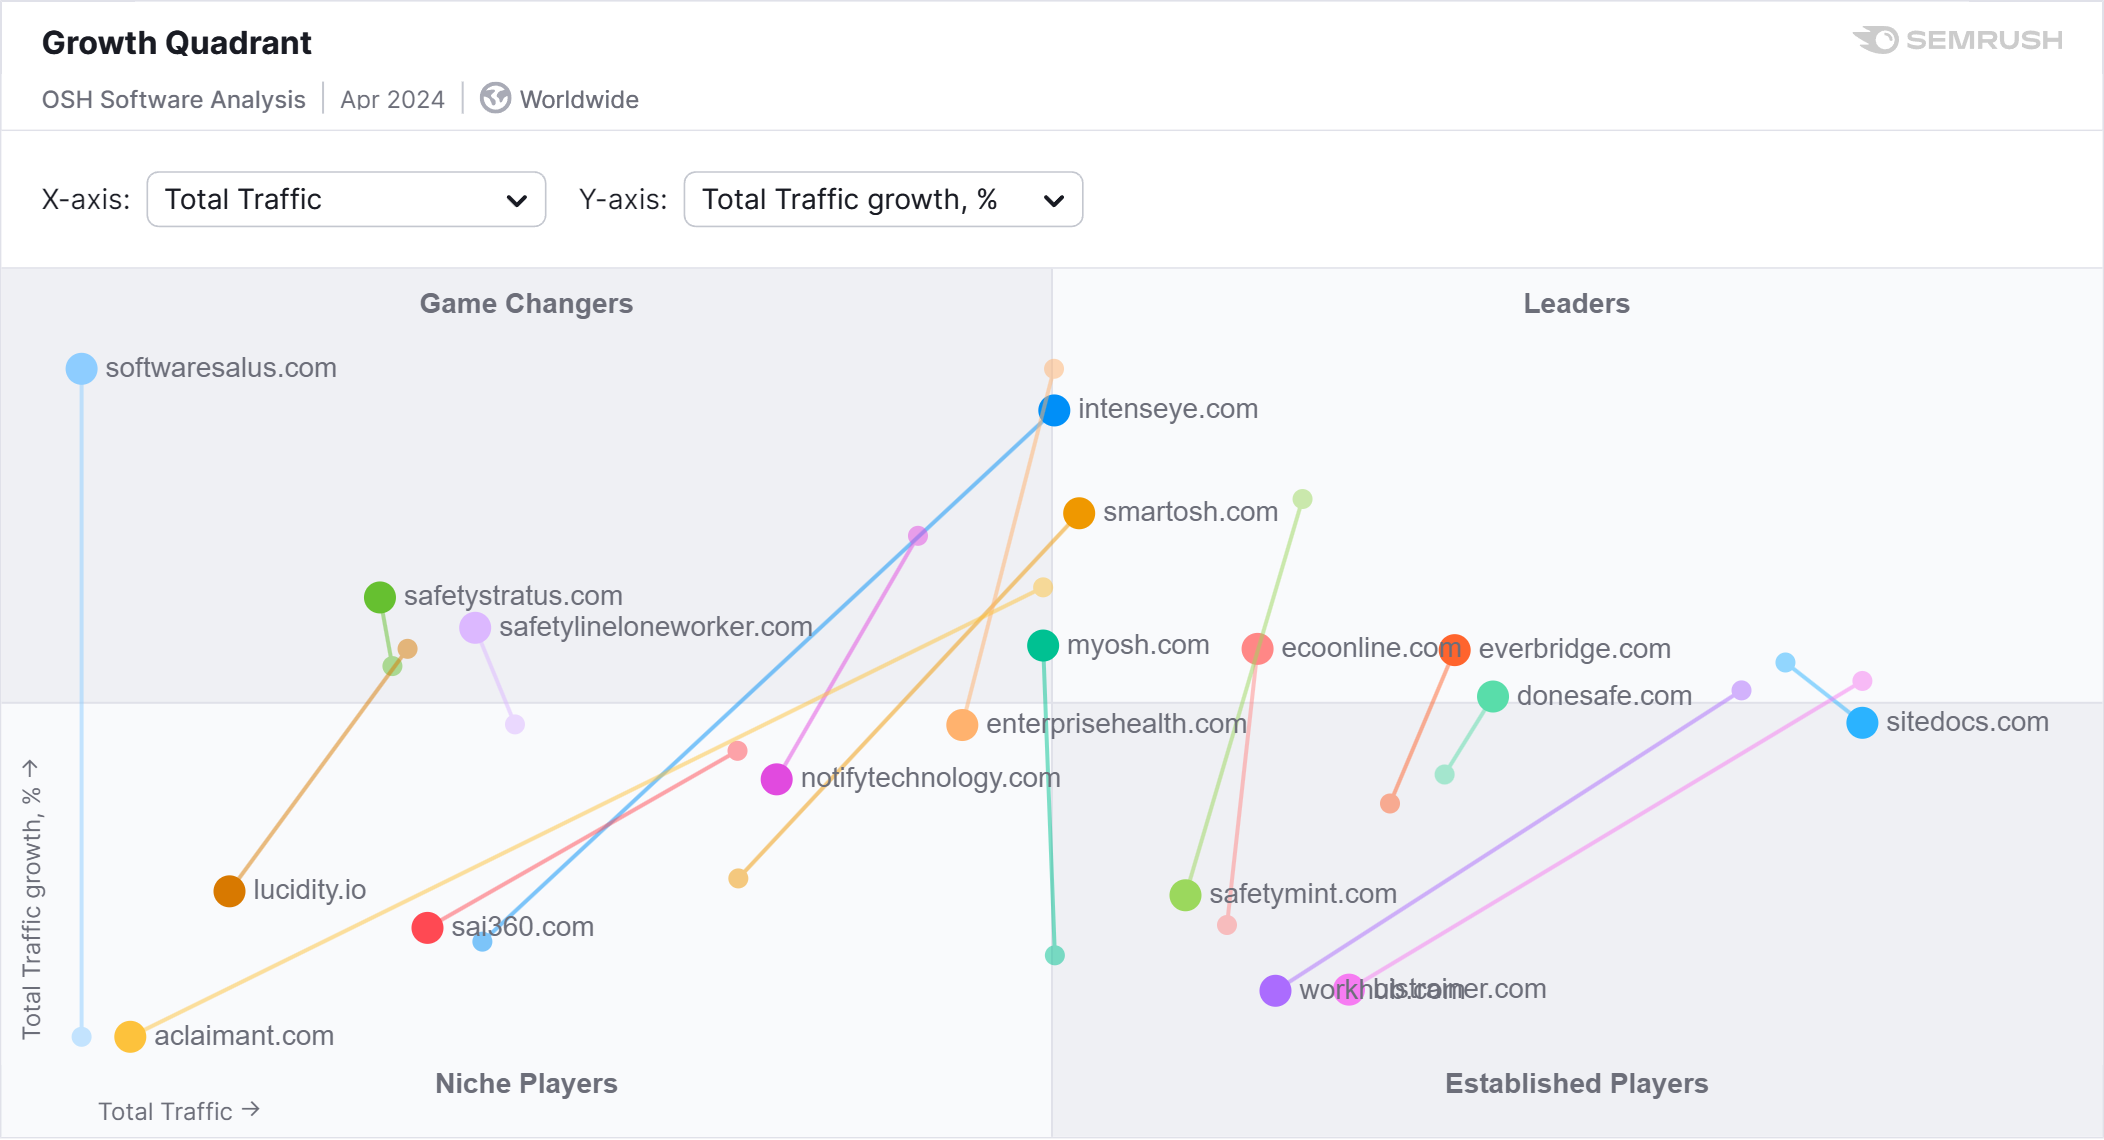
\includegraphics[width=0.95\linewidth]
        {images/marcopractico/planificacion/GrowthQuadrant.png}
    }
    \caption{Matriz de Competidores: \textit{OSH Software}}
    \vspace{-0.2cm}
	\footnotesize{Fuente: Elaborado por \cite{SEMrushMarketExplorer}.}
    \label{fig:MatrizCompetidores}
\end{figure}

En esta matriz, \textit{sitedocs} se encuentra claramente en la categoría de líderes, no solo por su alto volumen de tráfico, sino también por un crecimiento positivo. Destacan los casos de \textit{intenseye} y \textit{smartosh} que también están en la categoría de líderes, mostrando un crecimiento significativo desde la categoría de jugadores de nicho. Por otro lado, dominios como \textit{softwareasalus} están catalogados como agentes de cambio debido a su impresionante crecimiento en el tráfico, aunque su volumen total de tráfico sea menor. Los jugadores establecidos, como \textit{donesafe} y \textit{workhub}, tienen un alto volumen de tráfico pero un crecimiento más estable y menos pronunciado.\\ \indent
Se puede concluir, en primer lugar que los agentes de cambio, como \textit{softwareasalus}, aunque tienen menor volumen de tráfico, están creciendo rápidamente, lo que sugiere que nuevas empresas pueden irrumpir en el mercado con innovaciones significativas y atraer rápidamente a los usuarios. Además, los jugadores establecidos, con su tráfico consolidado pero crecimiento lento, representan una estabilidad en el mercado, ofreciendo una base de comparación para el rendimiento y las estrategias de retención de usuarios.

%---------------------------------------------------------------------------------------------
%---------------------------------------------------------------------------------------------
\section{Cronograma de actividades}
Como se puede apreciar en la Tabla \ref{tab:cronograma_proyecto}, asi como en el diagrama Gantt del apéndice \ref{sec:cronograma}, se presenta un cronograma que detalla las fases y actividades del proyecto, que se desarrolla desde el 1 de febrero del 2024 hasta el 29 de septiembre de 2024. El mismo, siguiendo la metodología PXP se divide en tres fases principales mas la adición de una cuarta a fines de evaluar el desempeño en actividad del producto. Estas etapas son: Definición de Requisitos, Planificación, Iteraciones de Desarrollo, y Cierre. Cada fase incluye entregables específicos y actividades que se ejecutarán en un periodo determinado para asegurar la implementación exitosa del sistema.

\begin{table}[htb]
    \caption{Cronograma del proyecto.}
    \label{tab:cronograma_proyecto}
    \centering
    \resizebox{\textwidth}{!}{%
    \begin{tabular}{|c|c|c|c|c|}
        \hline
        \rowcolor{lightgray} \textbf{Etapa} & \textbf{Tareas} & \textbf{Fecha de Inicio} & \textbf{Fecha de Fin} & \textbf{Dias} \\
        \hline 
        \rowcolor{lightgray} Def. Requisitos &  & 01/02/2024 & 10/05/2024 & 99 \\ \hline
        ~ & Entrega Marco Referencial & \multicolumn{2}{|c|}{15/03/2024} & 1 \\ \hline
        ~ & Entrega de avance & \multicolumn{2}{|c|}{03/05/2024} & 1 \\ \hline
        ~ & Defensa & \multicolumn{2}{|c|}{10/05/2024} & 1 \\ \hline
        \rowcolor{lightgray} Planificación &  & 15/03/2024 & 30/06/2024 & 107 \\ \hline
        ~ & Entrega de avance & \multicolumn{2}{|c|}{24/05/2024} & 1 \\ \hline
        ~ & Entrega de perfil & \multicolumn{2}{|c|}{07/06/2024} & 1 \\ \hline
        ~ & Defensa & \multicolumn{2}{|c|}{14/06/2024} & 1 \\ \hline
        ~ & Análisis de Procesos & 17/06/2024 & 23/06/2024 & 6 \\ \hline
        ~ & Diseño de Arq. & 24/06/2024 & 30/06/2024 & 6 \\ \hline
        \rowcolor{lightgray} Desarrollo &  & 01/07/2024 & 01/09/2024 & 62 \\ \hline
        ~ & Iteración 1 & 01/07/2024 & 21/07/2024 & 20 \\ \hline
        ~ & Iteración 2 & 22/07/2024 & 11/08/2024 & 20 \\ \hline
        ~ & Iteración 3 & 12/08/2024 & 01/09/2024 & 20 \\ \hline
        \rowcolor{lightgray} Cierre &  & 02/09/2024 & 29/09/2024 & 27 \\ \hline
        ~ & Preparación de Documentación  & 02/09/2024 & 08/09/2024 & 6 \\ \hline
        ~ & Capacitación de Usuarios & 09/09/2024 & 15/09/2024 & 6 \\ \hline
        ~ & Monitoreo Inicial y Ajustes & 16/09/2024 & 22/09/2024 & 6 \\ \hline
        ~ & Pruebas con Usuarios & 23/09/2024 & 29/09/2024 & 6 \\
        \hline
    \end{tabular}
    }
\end{table}

La primera fase, Definición de Requisitos, abarca desde el 1 de febrero hasta el 10 de mayo de 2024, e incluye entregas clave como el marco referencial, avances y la defensa del perfil del proyecto. La segunda fase, Planificación, se extiende desde el 15 de marzo hasta el 30 de junio de 2024, y cubre actividades como la entrega de avances adicionales, la entrega completa del perfil, la defensa final del perfil, el análisis de procesos y el diseño de la arquitectura de alto nivel. La tercera fase, Iteraciones de Desarrollo, se lleva a cabo del 1 de julio al 1 de septiembre de 2024, con tres iteraciones de desarrollo, cada una de tres semanas. Finalmente, la fase de Cierre y Evaluación Final, del 2 de septiembre al 29 de septiembre de 2024, incluye la preparación de documentación, capacitación de usuarios, monitoreo inicial y ajustes, y pruebas con usuarios.

En conclusión, el cronograma establece un plan detallado para la implementación del sistema automatizado de gestión de PGSST, asegurando que cada fase del proyecto se ejecute de manera organizada y meticulosa. Este enfoque estructurado permite abordar de manera efectiva los objetivos del proyecto, garantizando que todas las actividades necesarias se completen dentro de los plazos establecidos, lo que facilita un desarrollo coherente y exitoso del sistema que cumplirá con los estándares y requisitos normativos en Bolivia.

%---------------------------------------------------------------------------------------------
%---------------------------------------------------------------------------------------------
\section{Indice tentativo}
En esta sección se describen de forma detallada todos los capítulos a ser desarrollados en el proyecto de grado. En la introducción, se establecen los antecedentes de la problemática. Se plantea y define el problema a investigar, se delinean los objetivos generales y específicos, y se justifica la relevancia del mismo desde perspectivas legal, tecnológica y social. Además, se delimitan los límites y alcances de la investigación, proporcionando un marco contextual sólido para el desarrollo del proyecto.

El desarrollo del trabajo se fundamenta en el marco teórico y legal, donde se exploran conceptos fundamentales de salud y seguridad ocupacional, así como la legislación aplicable a la materia. Se abordan también metodologías de desarrollo de software, análisis y evaluación de software, y se profundiza en el campo de la inteligencia artificial, proporcionando un contexto amplio y diverso que sustenta la investigación los objetivos del proyecto.

Tras el marco practico en el que se resuelve el problema. Finalmente, se presentan las conclusiones derivadas del proyecto, se ofrecen recomendaciones pertinentes basadas en los hallazgos obtenidos, y se esbozan posibles líneas de trabajo. Este índice proporciona una guía clara y estructurada del contenido que se desarrollará a lo largo del trabajo, asegurando una presentación coherente y completa del proyecto.

\begin{enumerate}[label*=\arabic*.]
    \item \textbf{Introducción}
    \begin{enumerate}[label*=\arabic*.]
        \item \textbf{Antecedentes}
        \item \textbf{Planteamiento del Problema}
        \item \textbf{Definición del Problema}
        \item \textbf{Objetivos}
        \begin{enumerate}[label*=\arabic*.]
            \item Objetivo general
            \item Objetivos específicos
        \end{enumerate}
        \item \textbf{Justificación}
        \begin{enumerate}[label*=\arabic*.]
            \item Justificación legal
            \item Justificación tecnológica
            \item Justificación social
        \end{enumerate}
        \item \textbf{Delimitación}
        \begin{enumerate}[label*=\arabic*.]
            \item Límites
            \item Alcances
        \end{enumerate}
    \end{enumerate}
    \item \textbf{Marco teórico y legal}
    \begin{enumerate}[label*=\arabic*.]
        \item \textbf{Salud y Seguridad Ocupacional}
        \begin{enumerate}[label*=\arabic*.]
            \item Conceptos Fundamentales
            \begin{enumerate}[label*=\arabic*.]
                \item Seguridad Ocupacional
                \item Salud Ocupacional
                \item Higiene Ocupacional
                \item Enfermedad Ocupacional
                \item Sistema de Gestión de Riesgos Ocupacionales
            \end{enumerate}
            \item Accidentes e Incidentes Ocupacionales
            \item Factores de accidentes
            \begin{enumerate}[label*=\arabic*.]
                \item Actos Inseguros
                \item Condición Insegura
            \end{enumerate}
            \item Ingeniería de Seguridad
            \item Práctica de Seguridad
            \item Investigación de accidentes
            \item Peligro
            \item Riesgo
            \begin{enumerate}[label*=\arabic*.]
                \item Riesgo Físico
                \item Riesgo Mecánico
                \item Riesgo Químico
                \item Riesgo Biológico
                \item Riesgo Psicosocial
                \item Riesgo Ergonómico
                \item Riesgo Aceptable
            \end{enumerate}
            \item Condiciones de Trabajo
            \begin{enumerate}[label*=\arabic*.]
                \item Iluminación
                \item Estrés Térmico
                \item Sonometría
                \item Ventilación
                \item Señalización
                \item Ergonomía
                \item Equipo de Protección Personal (EPP)
                \item Comité Mixto
                \item Inspección de Salud y Seguridad en el trabajo
            \end{enumerate}
        \end{enumerate}
        \item \textbf{Legislación Aplicable a la SySO}
        \begin{enumerate}[label*=\arabic*.]
            \item Contexto Histórico
            \item Normativa obligatoria
            \begin{enumerate}[label*=\arabic*.]
                \item Constitución Política del Estado
                \item Ley General del Trabajo
                \item Reglamento de la Ley General de Trabajo
                \item Ley General de Higiene, Seguridad Ocupacional y Bienestar
                \item Disposiciones Complementarias
            \end{enumerate}
            \item Normativa voluntaria
            \begin{enumerate}[label*=\arabic*.]
                \item NB/ISO 62005:2005
                \item NB/ISO 55001:2005
                \item NB/ISO 51002:2012
                \item NB/ISO 7243:2018
                \item NB/ISO 45001:2018
                \item NB/ISO 51001:2022
                \item NB/ISO 58005:2022
                \item NB/ISO 11226:2022
            \end{enumerate}
        \end{enumerate}
        \item \textbf{Metodologías de Desarrollo de Software}
        \begin{enumerate}[label*=\arabic*.]
            \item Programación Extrema
            \item Programación Extrema Personal
            \begin{enumerate}[label*=\arabic*.]
                \item Técnica MoSCoW
            \end{enumerate}
        \end{enumerate}
        \item \textbf{Análisis y Evaluación de Software}
        \begin{enumerate}[label*=\arabic*.]
            \item Estándar ISO 25000:2014
            \item Método Objetivo-Pregunta-Métrica
        \end{enumerate}
        \item \textbf{Inteligencia Artificial}
        \begin{enumerate}[label*=\arabic*.]
            \item Aprendizaje
            \item Redes Neuronales
            \item Visión Computacional
            \item Procesamiento de Lenguaje Natural (PLN)
            \item Modelos de Lenguaje Multimodales
            \item Evaluación de Modelos
            \item Generación de Lenguaje Natural
            \item Generación de Descripciones de Imágenes
        \end{enumerate}
    \end{enumerate}
    \item \textbf{Marco Practico}
        \begin{enumerate}[label*=\arabic*.]
            \item Revisión de Requisitos
            \item Análisis de procesos actuales
            \item Establecimiento de arquitectura del sistema
            \begin{enumerate}[label*=\arabic*.]
                \item Alto nivel
                \item Detalle
                \item Base de Datos
            \end{enumerate}   
            \item Implementación del sistema
            \item Evaluación de la calidad del software
        \end{enumerate}
    \item \textbf{Marco Analítico}
        \begin{enumerate}[label*=\arabic*.]
            \item Resultados y Discusión
            \item Análisis de Costos
                \begin{enumerate}[label*=\arabic*.]
                    \item Costos de Desarrollo
                    \item Costos de Infraestructura
                    \begin{enumerate}[label*=\arabic*.]
                        \item Servidores y Almacenamiento
                        \item Red y Seguridad
                        \item Costos Totales de Infraestructura
                    \end{enumerate}
                    \item Gastos Legales
                    \item Inversión Total Inicial
                \end{enumerate}
            \item Evaluación de Proyecto de Inversión
            \begin{enumerate}[label*=\arabic*.]
                \item Comparación Costo Beneficio
                \item Valor Actual Neto
                \item Tasa Interna de Retorno
                \item Conclusión
            \end{enumerate}
            \item Análisis de Competidores
            \item Conclusión del capítulo
        \end{enumerate}
    \item \textbf{Marco Conclusivo}
        \begin{enumerate}[label*=\arabic*.]
            \item Conclusiones
            \item Recomendaciones
            \item Trabajos Futuros
        \end{enumerate}
    \item \textbf{Bibliografía, Apéndices y Anexos}
\end{enumerate}